
\section{Bodies and Particles}

Let body $\cB$ be an open, bounded subset of three-dimensional           
Euclidean space $\realnsd$ with boundary $\partial \cB$.                 
The number of space dimensions, $\nsd$, is assumed equal                    
to three unless stated otherwise.
The boundary is decomposed within a particular space dimension into         
two non-overlapping subdomains, $\Gamma_u$ and $\Gamma_{\sigma}$        
where displacements or tractions are prescribed.  Thus                      
$\partial \Omega = \Gamma_u \union \Gamma_{\sigma}$ and 
$\Gamma_u \intersection \Gamma_{\sigma} = \emptyset$.           
Set closure is denoted                                                      
$\bar{\cB} = \cB \union \partial \cB$.                             
Let the body be composed of a closed set of particles with 
coordinates $\vX$ in the reference configuration.  The particle
has coordinates $\vX = \{X_1, X_2, X_3\}^T$ as measured from
some origin $O$ in the dextral, orthonormal inertial reference
from $\vE_1, \vE_2, \vE_3$.


\section{Motion}
Let the arbitrary time interval be defined as
$\interval \defe [t_0,T]$.\footnote{Note that $t_0$, while
typically zero, may be any real number.}  
Let the motion, a one parameter family of configurations, 
$\vvarphi : \cB \times \interval \mapsto \realthree$ 
map the material particle
$\vX$ into the current configuration $\vx$ such that
\be
\vx = \vvarphi(\vX,t) = \vvarphi_t(\vX).
\ee

A motion evaluated
at a particular time $t \in \interval$ 
is referred to as a configuration or
placement.  To each configuration, we assign a displacement
field $\vu: \cB \mapsto \realthree$ such that 
\be
\vu(\vX,t) = \vvarphi(\vX,t) - \vX.
\label{eq:displacement}
\ee
Thus, the current configuration $\vvarphi$ is simply a function 
of the original
placement $\vX$, 
plus a displacement $\vu$, which is {\bf function}
of placement $\vX$ and time $t$:
\be
\vvarphi(\vX,t) = \vX + \vu(\vX,t).
\label{eq:displacement_vvarphi}
\ee
It is important to
emphasize that the displacement remains a function $\vu = \vu(\vX, t)$
of reference configuration $\vX$ and time $t$.  The displacement
function $\vu$ is not a simple (constant) displacement, which 
we refer to as ``offset'' in Section~\ref{section:offset}.

\subsection{Linear Motions}
In this section, we consider the equation of a line
\be
y = f(x) =  m x + b,
\ee
as inspiration for writing (\ref{eq:displacement_vvarphi}) 
as\footnote{
For the time being, we will not be concerned with time $t$, so we
eliminate it from our notation for the sake of brevity.}
\be
\vx = \vvarphi(\vX) = 
\underbrace{\; \tMbold \; \vX \;}_{\text{linear in $\vX$}} 
+ 
\underbrace{\vb}_{\text{constant}} 
\stackrel{\mbox{\scriptsize set}}{=} \vX + \vu(\vX).
\ee
Then the displacement can be written as
\begin{align}
 \vu(\vX) &= \tMbold \vX + \vb - \vX, \\
          &= (\tMbold - \vid) \vX + \vb. \label{eq:displacement_M}
\end{align}
In the following sections, we will be exploring the
effect of ``slope'' $\tMbold$ and 
``intercept'' $\vb$ on displacements $\vu$. 
To explore some motions, we shall consider the two-dimensional
body shown in Fig.~\ref{fig:configuration_reference}.  

\begin{figure}[h!]
  \caption{Reference configuration of a body defined by particles
  with $X_1 \in [-1, 1]$ and $X_2 \in [-1, 1]$.  With the 
  continuum body is composed of an infinite number of particles, 
  only nine particles are shown for the sake of simplicity.  Eight of
  the nine particles shown are on the boundary of the body, and a 
  single particle at the geometric center is the ninth particle.}
  \begin{center}
    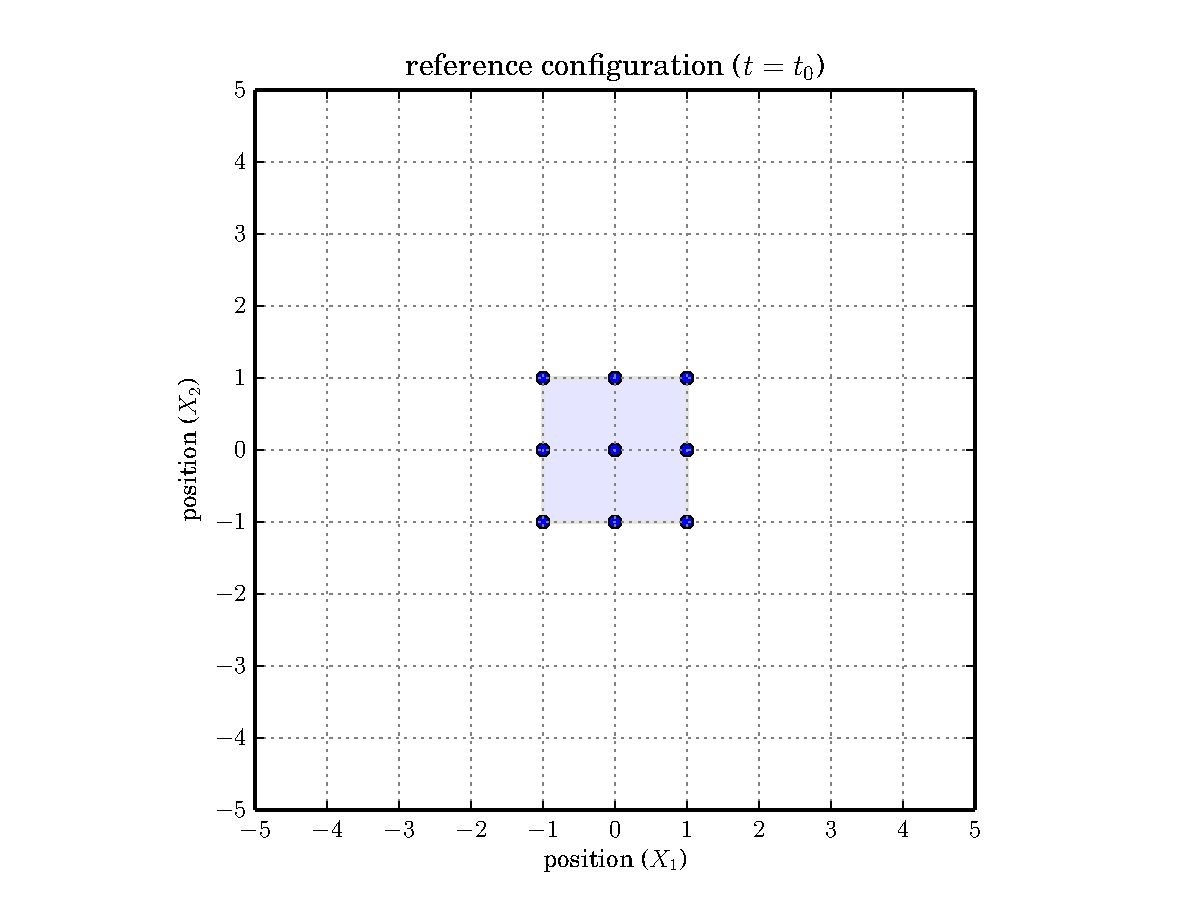
\includegraphics[width=\textwidth]{fig/configuration_reference.pdf}
  \end{center}
  \label{fig:configuration_reference}
\end{figure}

The most elementary displacement is homogeneous, when 
$\tMbold = \vid$ 
and
$\vb = \vzero$, then $\vu = \vzero$.
In this case $\vvarphi = \vX$ and the motion is trivial (and
uninteresting).  Nonetheless, this is a simple first case to consider.

\subsection{Offset}
\label{section:offset}
Next, consider $\vb \neq \vzero$, while
retaining $\tMbold = \vid$.   For the concrete example 
in Fig.~(\ref{fig:configuration_current}), let 
$\vb = \langle b_1, b_2 \rangle\transpose = 
\langle 3, 2 \rangle\transpose$.
In this case, we see the placement $\vvarphi$ moves right and up
on the page, relative to the reference configuration $\vX$, by 
an amount of 3 and 2, respectively.
\begin{figure}[htb]
  \caption{Current configuration shown in red, with reference 
  configuration shown in blue and retained for context.}
  \begin{center}
    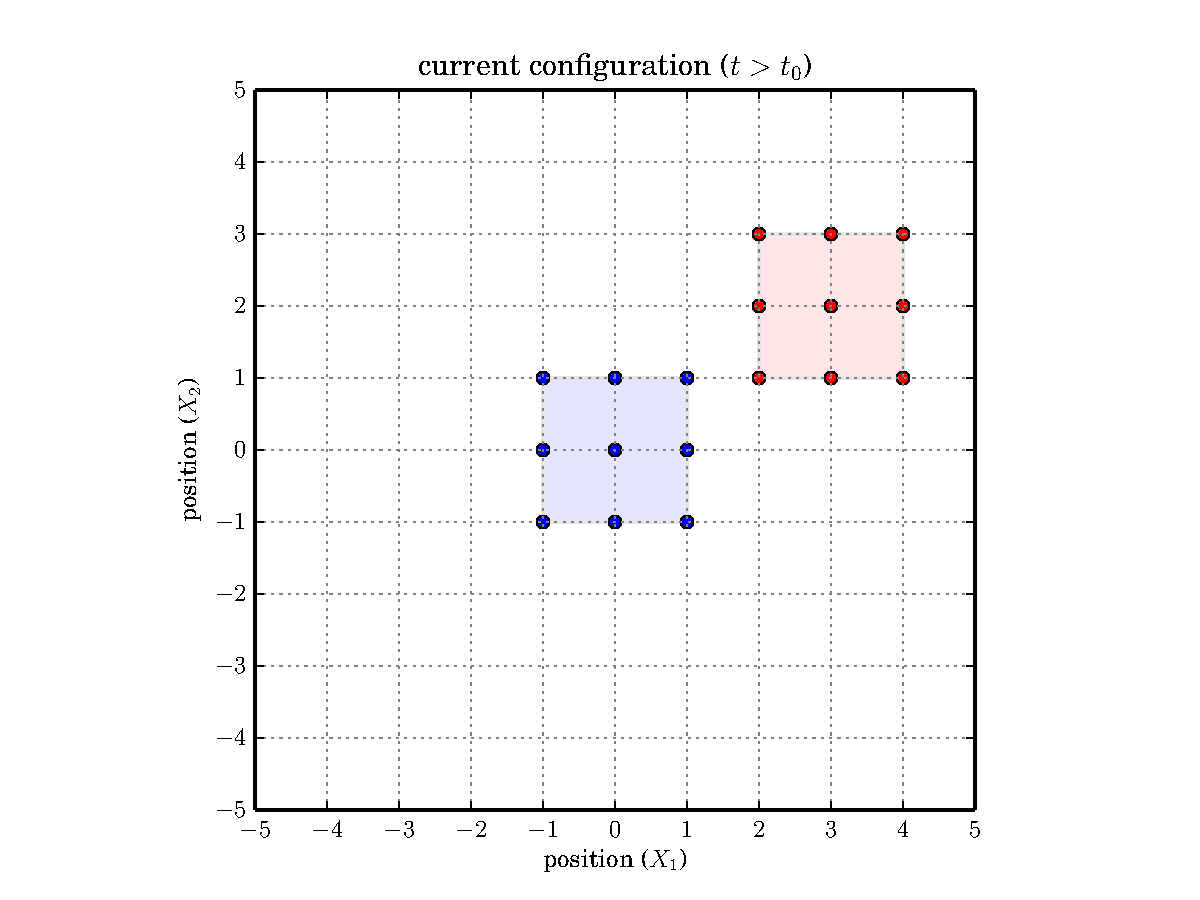
\includegraphics[width=\textwidth]{fig/configuration_current.pdf}
  \end{center}
  \label{fig:configuration_current}
\end{figure}


\clearpage
\subsection{Stretch}
Consider now $\tMbold = \lambda \vid$ and $\vb = \vzero$.  
This describes {\bf volumetric} response, also known 
as a {\bf dilitational} response.  The parameter $\lambda \in \real$
causes the current configuration to change volume as
\begin{itemize}
 \item $\lambda > 0$ expansion,
 \item $\lambda = 0$ identity,
 \item $\lambda < 0$ contraction.
\end{itemize}
Notice that $\lambda$ describes the ``slope'' of the mapping from
reference to current configurations.  In the case that $\lambda \rightarrow
+\infty$, the volume grows infinite.  In the case that $\lambda \rightarrow
-\infty$, the volume grows to zero.
For concreteness, consider $\lambda = 2$.  The volumetric expansion
is shown in Fig.~\ref{fig:configuration_volumetric}.

\begin{figure}[htb]
  \caption{Current configuration shown in red, with reference 
  configuration shown in blue and retained for context.}
  \begin{center}
    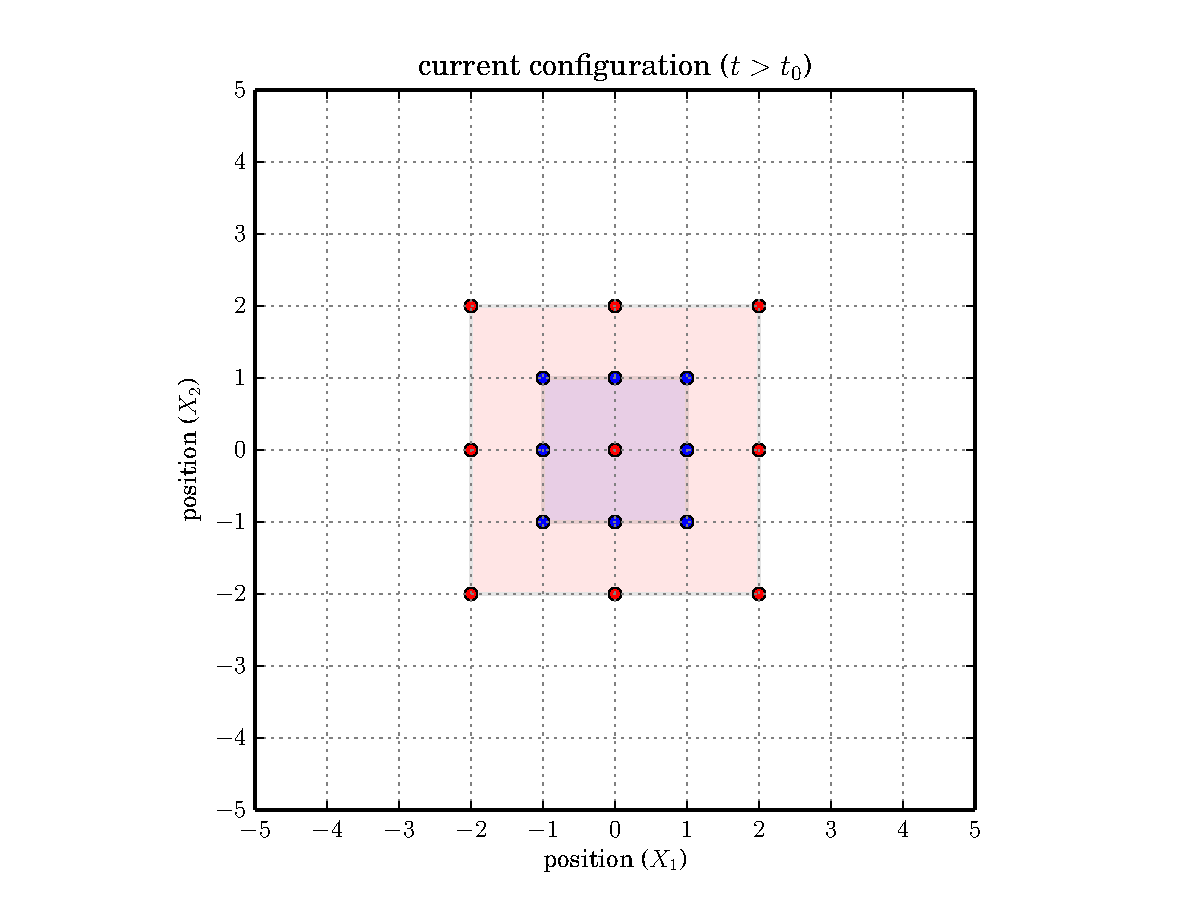
\includegraphics[width=\textwidth]{fig/configuration_volumetric.pdf}
  \end{center}
  \label{fig:configuration_volumetric}
\end{figure}

The area in the reference configuration was $2 \times 2 = 4$, 
whereas the area in the current configuration was $4 \times 4 = 16$.   


Next consider a slightly different form of $\tMbold$, such that
\be
 \tMbold 
 = 
 \left[
 \begin{tabular}{cc}
  $\lambda_1$ & 0 \\
  0 & $\lambda_2$
 \end{tabular}
 \right].
\ee
We keep the offset as $\vb = \vzero$.

For concreteness, consider $\lambda_1 = 2$
and $\lambda_2 = \half$.   The combined expansion and compression
is shown in Fig.~\ref{fig:configuration_stretch}.

\begin{figure}[htb]
  \caption{Current configuration shown in red, with reference 
  configuration shown in blue and retained for context.}
  \begin{center}
    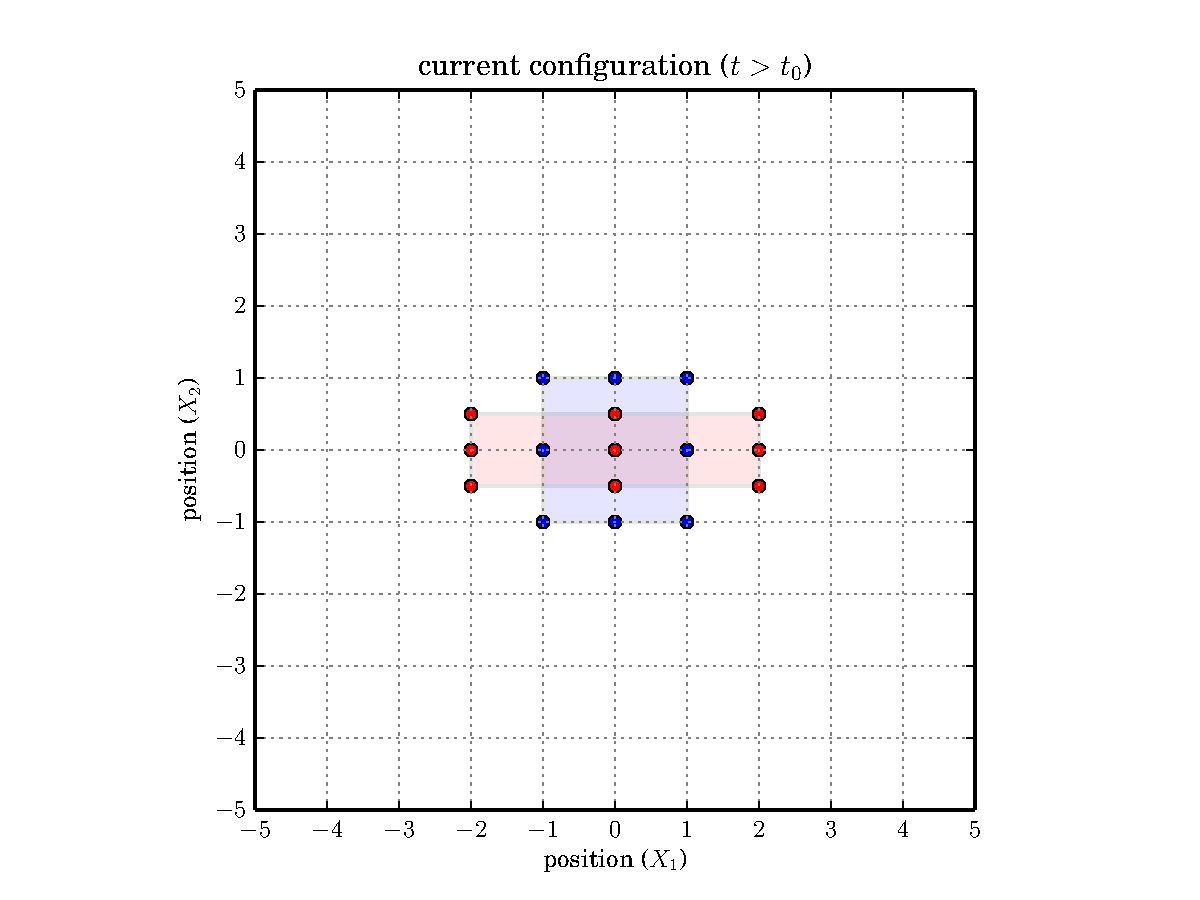
\includegraphics[width=\textwidth]{fig/configuration_stretch.pdf}
  \end{center}
  \label{fig:configuration_stretch}
\end{figure}

The area in the reference configuration was $2 \times 2 = 4$, 
whereas the area in the current configuration was $4 \times 1 = 4$.   
Out of coincidence, we have chosen stretches along the 
two axes such that the area does not change although the dimensions
and thus shape have changed.  This is an example of an 
{\bf isochoric} motion.  The roots {\em iso- (equal)} and {\em choro- (space)} 
describe a process from initial state $0$ to final state $1$
where the volume remains constant.  

Now, the motion as we have described it, doesn't yet show the {\em path}
taken between the reference and current configuration.  To 
get that detail, we would need to introduce the time parameter $t$, 
which we have suppressed for now.  
However, if we were to say the time interval is simply two points 
$t_0$ and $t_1$, we can create (the rather course) path between these
two states $0$ and $1$, and connect with the isochoric process
$PV$ diagram in thermodynamics, shown in Fig.~\ref{fig:PV_isochoric}.

\begin{figure}[htb]
  \caption{Isochoric process from initial state (reference configuration) $0$ to
  final state (current configuration) $1$.}
  \begin{center}
    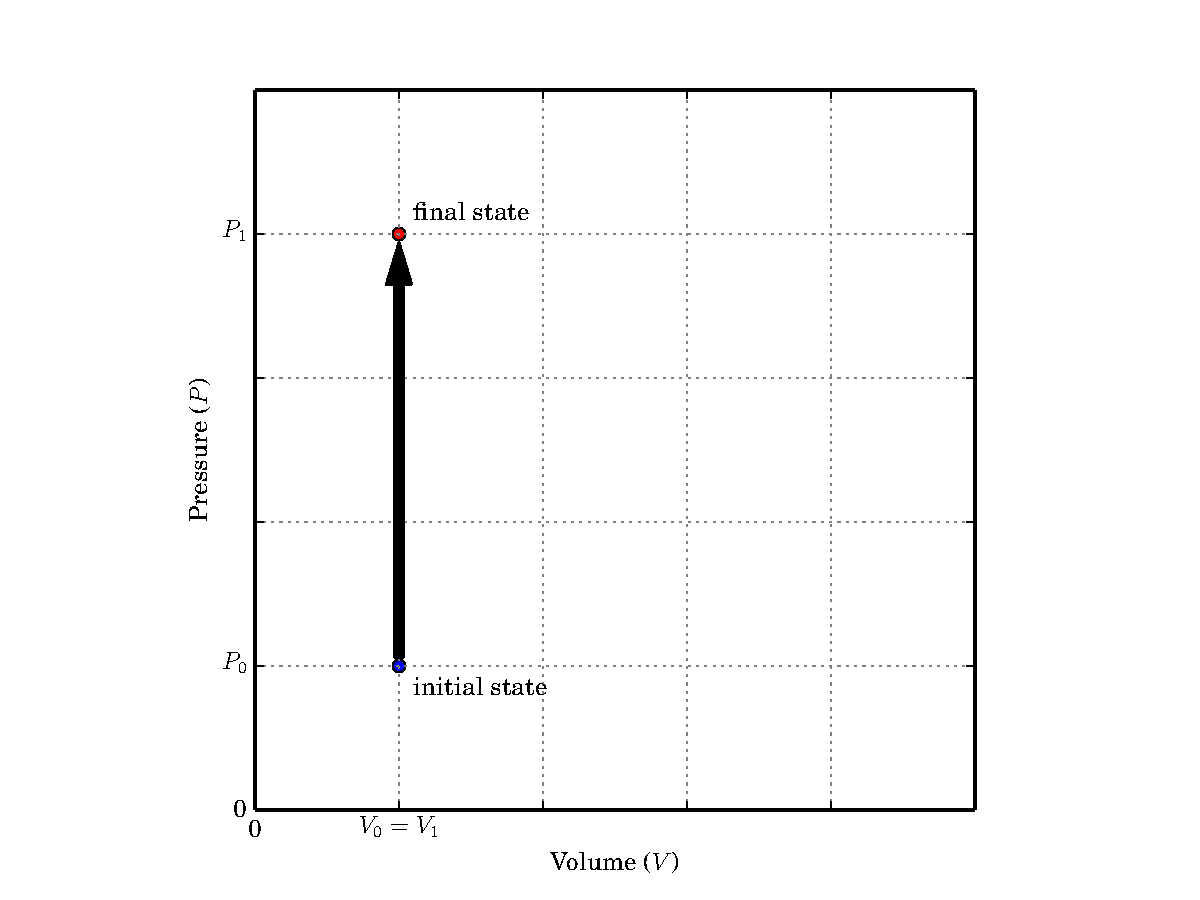
\includegraphics[width=\textwidth]{fig/PV_isochoric.pdf}
  \end{center}
  \label{fig:PV_isochoric}
\end{figure}

We have yet to introduce and define pressure $P$, so this 
connection may be tenuous at the moment.  Nonetheless, we
introduce this connection now to motivate the single idea that
isochoric motions will play an important role in our later work.

\subsection{Rotation}

\section{Deformation Gradient}
To each configuration, we define a deformation gradient 
$\tFbold: \cB \times \interval \mapsto \Mthreeplus$ 
such that
\begin{equation}
\tFbold 
\defe 
\Grad \vvarphi
\;\; \Longleftrightarrow \;\;
\tF_{iJ} 
\defe 
\frac{\partial \varphi_i}{\partial X_J}.
\label{eq:deformation_gradient}
\end{equation}
Remarks:
\begin{itemize}
\item Lower case indices represent components of tensors in the
current configuration whereas upper case indices represent
components of tensors in the reference configuration.  Real, 
square matrices of dimension three and positive determinants
are denoted $\Mthreeplus$.  
\item We define gradients taken in the reference configuration 
as $\Grad(\cdot) = \partial (\cdot) / \partial X_J$ 
to distinguish from gradients taken in the current
configuration, denoted simply as $\grad(\cdot) = 
\partial (\cdot) / \partial x_j$.
\item All configurations must be admissible in the sense that the Jacobian
of the deformation $J$ much be positive
\begin{equation}
 J \defe \det \tFbold > 0.
\end{equation}
This requirement keeps the deformations from mapping the body to
a single, infinitesimally small point ($J=0$) or turning the
body inside-out ($J<0$).  
\end{itemize}

From the displacement field in 
(\ref{eq:displacement}), we see that 
the relationship between the displacement gradient and the 
deformation gradient is given by
\be
\Grad \vu = \Grad \vvarphi - \vid = \tFbold - \vid.
\ee

\section{Strain}
\subsection{Right Cauchy-Green}
A standard strain measure is the right Cauchy-Green
strain tensor
\begin{equation}
 \tCbold 
 \defe 
 \tFbold\transpose \tFbold
 \;\; \Longleftrightarrow \;\;
 \tC_{IJ} 
 \defe 
 \tF_{Ii} \; \tF_{iJ}. 
\end{equation}
The right Cauchy-Green strain tensor $\tCbold$ gets its name from the 
fact that the deformation gradient $\tFbold$ sits to the right.  
Note that this strain tensor is defined in the reference configuration.
The right Cauchy-Green strain tensor can be written
explicitly as reference gradients of the motion 
$\vvarphi$ or displacement $\vu$:
\begin{align}
\tCbold &\overset{(\ref{eq:deformation_gradient})}{=} 
(\Grad \vvarphi)\transpose \Grad \vvarphi \nonumber \\
    &= (\Grad \vu + \vid)\transpose (\Grad \vu + \vid) \nonumber \\
    &= (\Grad \vu)\transpose\Grad \vu + \Grad \vu + (\Grad \vu)\transpose 
    + \vid
    \label{eq:C_in_terms_of_u}
\end{align}

\subsection{Left Cauchy-Green}
In contrast, a left Cauchy-Green
strain tensor $\tbbold$ can be defined with the 
deformation gradient $\tFbold$
sitting on the left.
\be
 \tbbold \defe \tFbold \tFbold\transpose
 \;\; \Longleftrightarrow \;\;
 \tb_{ij} \defe \tF_{iJ} \; \tF_{Jj}.
 \label{eq:left_cauchy_green}
\ee
Note that this strain measure is defined in the current 
configuration.

\subsection{Lagrangian (Green) Strain Tensor}
The Lagrangian (Green) strain tensor,
\begin{equation}
 \tEbold 
 \defe
 \half (\tCbold - \vid)
 \;\; \Longleftrightarrow \;\;
 \tE_{IJ} 
 \defe 
 \half(\tC_{IJ} - \delta_{IJ}),
\end{equation}
is closely related to the right Cauchy-Green strain tensor
and is often used in defining constitutive
law relationships because the measure, when linearized
about the reference configuration, coincides with the
small strain tensor of linear deformation elasticity, 
denoted~$\ve{\epsilon}$ and defined in (to come).
This relationship can be seen as follows:
\begin{align}
 2 \tEbold 
     &\overset{(\ref{eq:C_in_terms_of_u})}{=} 
     (\Grad \vu)\transpose \Grad \vu + 
     \Grad \vu + (\Grad \vu)\transpose + \vid - \vid,
     \label{eq:E_expanded} \\
 %\ve{\epsilon}  
 2 \tEbold_{\tiny \mbox{LIN}}
     %&\overset{\tiny \mbox{LIN}}{=} 
     &= 
     \Grad \vu + (\Grad \vu)\transpose,
     \label{eq:small_strain}
\end{align}
where the higher-order (first) term in (\ref{eq:E_expanded}) is set
to zero to achieve (\ref{eq:small_strain}).

\subsection{Eulerian (Almansi) Strain Tensor}
The Eulerian (Almansi) strain tensor,
\be
 \tebold 
 \defe 
 \half (\vid - \tbbold^{-1} )
 \;\; \Longleftrightarrow \;\;
 \te_{ij} 
 \defe 
 \half \left(\delta_{ij} - (\tb_{ij})^{-1}\right),
\ee
can likewise be used to approximate the small strain tensor
$\ve{\epsilon}$ by combining (\ref{eq:left_cauchy_green}) and
(\ref{eq:deformation_gradient}) as follows:
\begin{align}
 2 \tebold &=
     \vid - \left[ \Grad \vvarphi 
     (\Grad \vvarphi)\transpose \right]^{-1} \nonumber \\
     &= 
     \delta_{ij} 
       - \left[ \frac{\partial \varphi_i}{\partial X_J}
                \frac{\partial \varphi_j}{\partial X_J}
         \right]^{-1} % \nonumber \\
     =
      \delta_{ij} 
       - \left[ \frac{\partial X_J}{\partial \varphi_i}
                \frac{\partial X_J}{\partial \varphi_j}
         \right] 
	    \nonumber \\ 
     &\overset{(\ref{eq:displacement})}{=}
      \vid 
       - \left[
                (\vid - \grad \vu) (\vid - \grad \vu)\transpose
         \right]
	   \nonumber \\ 
     &=
     \grad \vu + \grad \vu\transpose - 
     \grad \vu \grad \vu\transpose 
     \label{eq:b_expanded} \\
 %\ve{\epsilon}  
 2 \tebold_{\tiny \mbox{LIN}} 
     %&\overset{\tiny \mbox{LIN}}{=} 
     &=
     \grad \vu + (\grad \vu)\transpose,
     \label{eq:small_strain_two}
\end{align}
where higher-order (quadratic) term in (\ref{eq:b_expanded}) is set
to zero to achieve (\ref{eq:small_strain_two}).

\subsection{When Strains are Small}

\subsection{Seth-Hill Strain Tensor Family}
Seth and Hill showed that the 
Lagrangian (Green) and Eulerian (Almansi)
strain tensors are special cases of the so-called
Seth-Hill family of strain measures, defined as
\be
 \tEbold_{(m)} \defe \frac{1}{2 m}
 \left(\tUbold^{2 m} - \vid \right)
 = 
 \frac{1}{2 m} 
 \left(\tCbold^m - \vid \right).
\ee
Then
\begin{align}
 \tEbold_{(1)} = 
 \half \left(\tUbold^{2} - \vid \right) = 
 \half \left(\tCbold - \vid \right) 
 & \hspace{1cm} \mbox{{\bf Lagrangian (Green)}}, \\
 \tEbold_{(1/2)} = 
 \left(\tUbold - \vid \right)  = 
 \left(\sqrt{\tCbold} - \vid \right) 
 & \hspace{1cm} \mbox{{\bf Biot}}, \\
\tEbold_{(0)} = 
 \ln\tUbold   = 
 \half \ln\tCbold
 & \hspace{1cm} \mbox{{\bf Logarithmic, Natural, True, Hencky}}, \\
\tEbold_{(-1)} = \half 
 \left(\vid - \tUbold^{(-2)} \right) 
 & \hspace{1cm} \mbox{{\bf Eulerian (Almansi)}}.
\end{align}


\subsubsection{The Linearized Lagrangian (Green) Strain Tensor 
Creates Nonzero Strains under Rigid Body Rotations}

Because it takes on nonzero values under finite rotation,
the linearized strain tensor 
should not be used for geometrically nonlinear analysis.
These nonzero values are completely artificial and strictly
an artifact of using a linear strain definition with
geometrically nonlinear motions.   This result is shown as follows:

Let $\tRbold = \tRbold(t)$ be a two-dimensional, 
rigid body rotation parameterized by time $t$
and scaled by constant $\omega = 2 \pi$~radians per second.  
Then, the motion $\vvarphi$ of a body can be written as
\be
 \vvarphi(\vX, t) = \tRbold(t) \vX 
 \;\; \Longleftrightarrow \;\;
 \left\{
 \begin{tabular}{c}
 $x_1$ \\
 $x_2$
 \end{tabular}
 \right\}
 = 
 \left[
 \begin{tabular}{rr}
 $\cos \omega t$ & $\sin \omega t$ \\
 $-\sin \omega t$ & $\cos \omega t$ 
 \end{tabular}
 \right]
 \left\{
 \begin{tabular}{c}
 $X_1$ \\
 $X_2$
 \end{tabular}
 \right\}.
\ee
Then the deformation gradient $\tFbold = \tFbold(t)$ is a function of time
alone,
\be
 \tFbold(t)
 \;\; \Longleftrightarrow \;\;
 \tF_{iJ} 
 = 
 \left[
 \begin{tabular}{rr}
 $\tF_{11}$ & $\tF_{12}$ \\
 $\tF_{21}$ & $\tF_{22}$ 
 \end{tabular}
 \right]
 =
 \left[
 \begin{tabular}{rr}
 $\cos \omega t$ & $\sin \omega t$ \\
 $-\sin \omega t$ & $\cos \omega t$ 
 \end{tabular}
 \right].
\ee
The linearized strain tensor is found to be 
\begin{align}
 2 \tEbold_{\tiny \mbox{LIN}}
 &= \Grad \vu + (\Grad \vu)\transpose, \\
 &= \tFbold - \vid + 
     \left(\tFbold - \vid \right)^T, \\
 &= \tF_{iJ} - \delta_{iJ} + \tF_{Ji} - \delta_{Ji}, \\ 
 &= 
 \left[
 \begin{tabular}{rr}
 $\cos \omega t$ & $\sin \omega t$ \\
 $-\sin \omega t$ & $\cos \omega t$ 
 \end{tabular}
 \right]
 +   
 \left[
 \begin{tabular}{rr}
 $\cos \omega t$ & $-\sin \omega t$ \\
 $\sin \omega t$ & $\cos \omega t$ 
 \end{tabular}
 \right]
 -   
 \left[
 \begin{tabular}{rr}
 $2$ & $0$ \\
 $0$ & $2$ 
 \end{tabular}
 \right], \\
 &=
 2 \left( \cos \omega t - 1 \right) \vid.
\end{align}
Now, for small angles, $\omega t \approx 0$, which is
for small deviations $x_1 \approx X_1$, $x_2 \approx X_2$, then
$\tEbold_{\tiny \mbox{LIN}} = \ve{0}$ for rigid body rotations.
However, for arbitrary finite angles, $\omega t \neq 0$,
and the linearized strain tensor
$\tEbold_{\tiny \mbox{LIN}}$ reports nonzero strain for rigid
body rotations, which is nonsensical.

A correct strain tensor will report zero strain for rigid body
rotations.  One such strain tensor is the fully nonlinear Lagrangian
(Green) strain tensor.  This result is shown as follows:
\begin{align}
 2 \tEbold &= \tFbold\transpose\tFbold - \vid \\
 &= 
 \left[
 \begin{tabular}{rr}
 $\cos \omega t$ & $-\sin \omega t$ \\
 $\sin \omega t$ & $\cos \omega t$ 
 \end{tabular}
 \right]
 \left[
 \begin{tabular}{rr}
 $\cos \omega t$ & $\sin \omega t$ \\
 $-\sin \omega t$ & $\cos \omega t$ 
 \end{tabular}
 \right]
 -   
 \left[
 \begin{tabular}{rr}
 $1$ & $0$ \\
 $0$ & $1$ 
 \end{tabular}
 \right] = \ve{0}. 
\end{align}

\section{Stress}

\section{Hyperelasticity}


